\documentclass[
	fontsize=11pt,
	paper=a4,
	pagesize=auto,
	parskip=half,
	titlepage=on,
	ngerman
]{scrartcl}

\usepackage[T1]{fontenc}
\usepackage[utf8]{inputenc}
\usepackage{float}
\usepackage{subcaption}
\usepackage[final]{graphicx}
\graphicspath{ {./images/} }
\usepackage{babel}
\usepackage{amsmath}
\usepackage{siunitx}
\sisetup{locale=DE}
\usepackage{lmodern}
\usepackage{url}
\usepackage{microtype}
\usepackage[shortlabels]{enumitem}
\usepackage[hidelinks]{hyperref}
\usepackage{float}
\usepackage{multicol}
\usepackage{blindtext}

\renewcommand{\labelenumi}{\Roman{enumi}.}
\renewcommand{\labelenumii}{\arabic{enumii}.}

\begin{document}

\title{Protokoll zur Leiterschaukel}
\subtitle{durchgeführt am 14.06.2024}
\author{Erik Graumann}
\date{\today}
\maketitle
\newpage

\tableofcontents
\newpage

\section{Aufbau}

\begin{figure}[h]
	\begin{subfigure}{.5\textwidth}
		\centering
		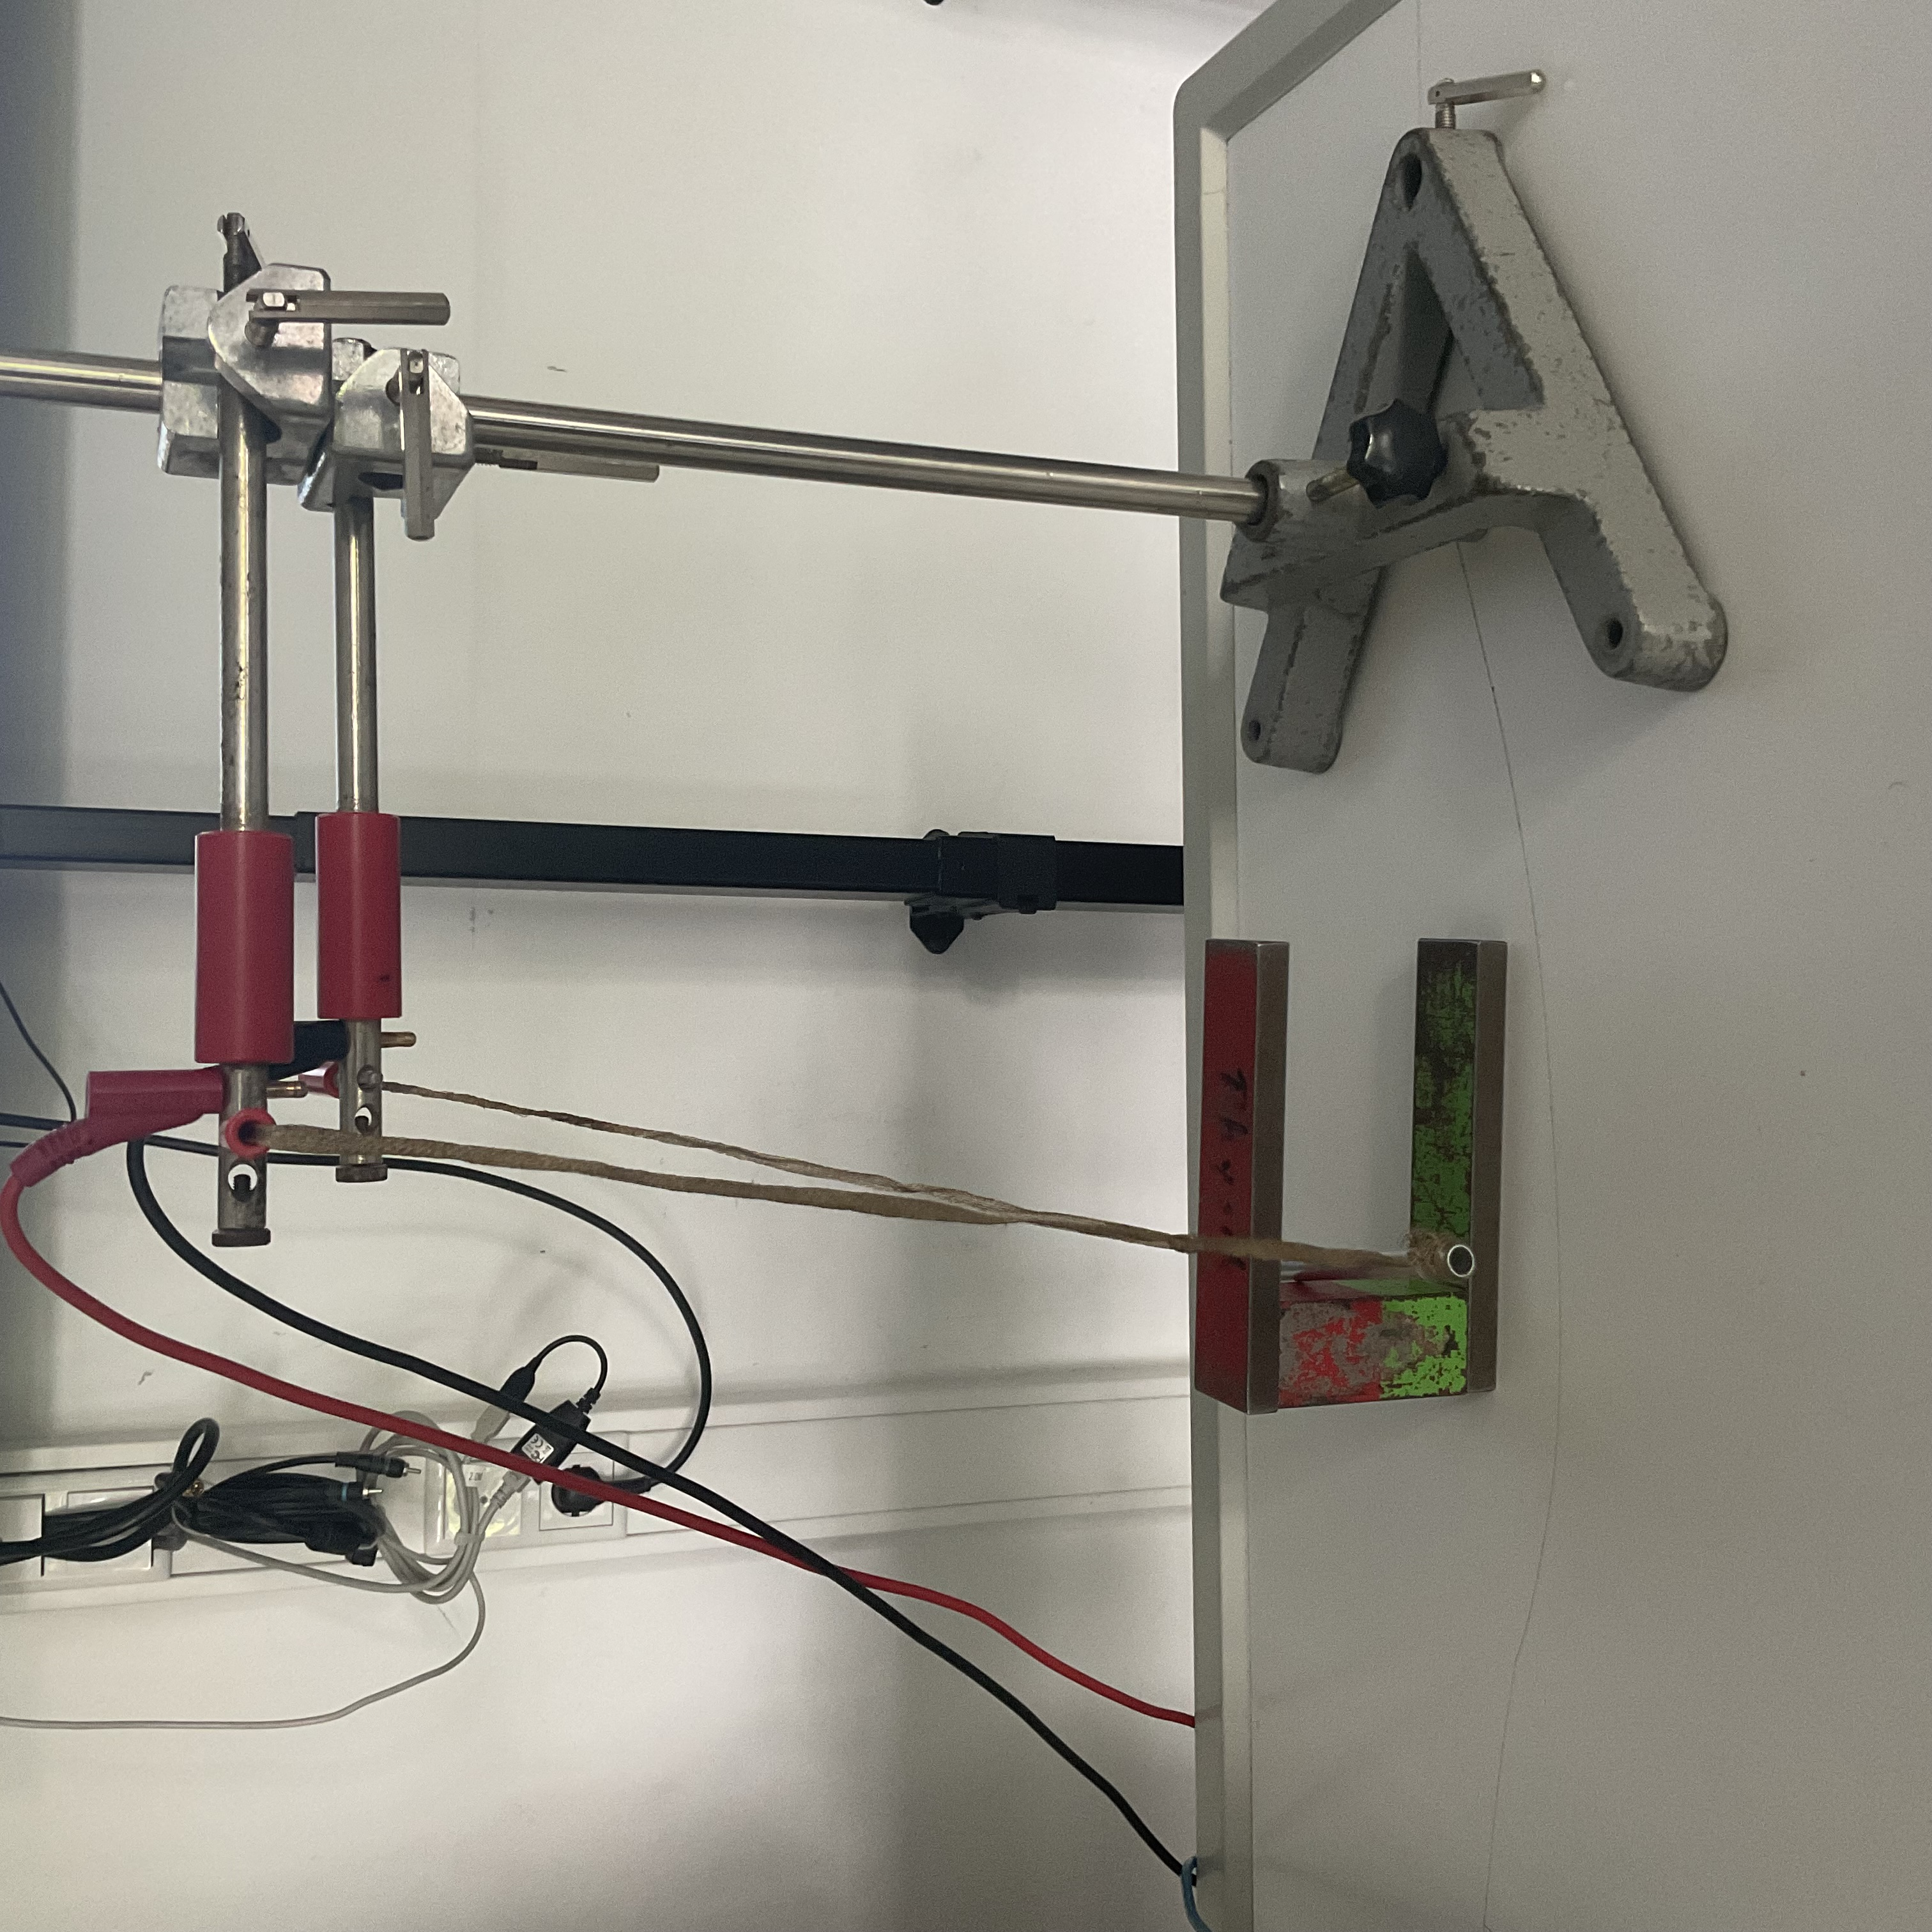
\includegraphics[width=.8\linewidth, angle=270]{IMG_1459.jpeg}
		\caption{Fall 1}
		\label{fig:fall1}
	\end{subfigure}%
	\begin{subfigure}{.5\textwidth}
		\centering
		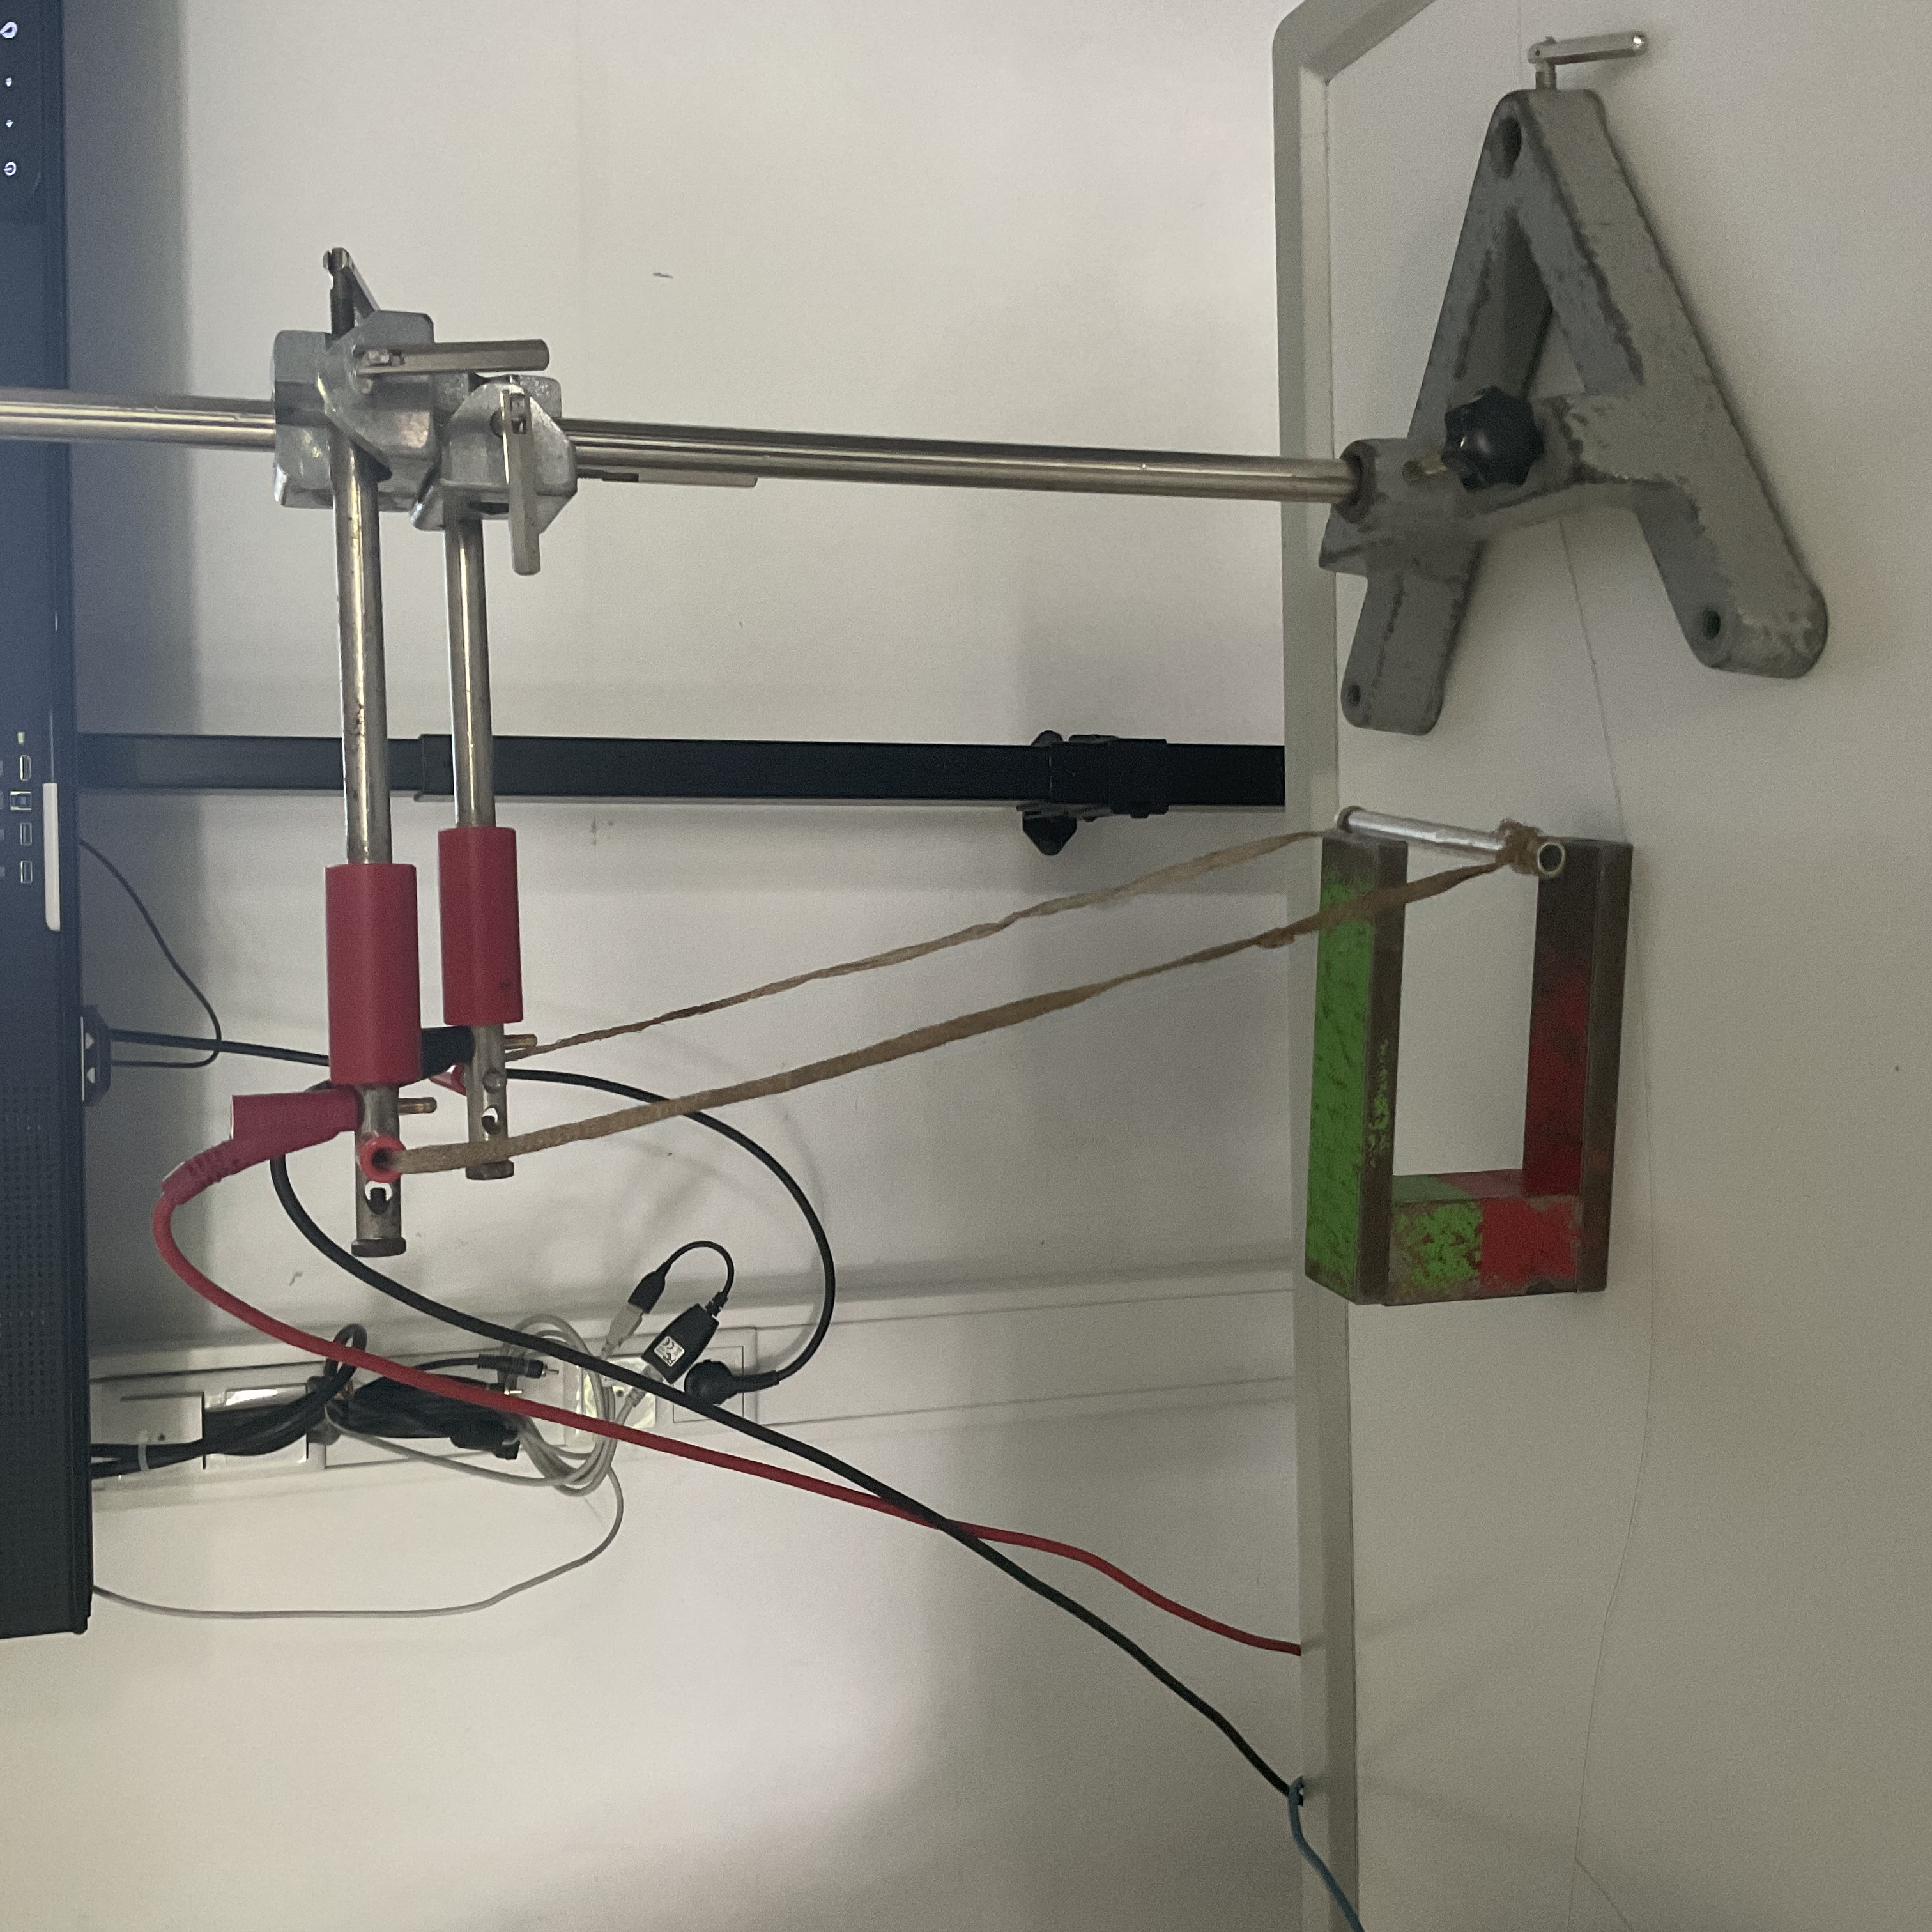
\includegraphics[width=.8\linewidth, angle=270]{IMG_1457.jpeg}
		\caption{Fall 2}
		\label{fig:fall2}
	\end{subfigure}
	\caption{Aufbau und Beobachtungen}
	\label{fig:aufbau}
\end{figure}

Es wurde ein Leiter zwischen zwei Stative aufgehängt. An den Aufhängungen des Leiters wurde ein Netzteil angeschlossen, sodass mit dem Leiter ein geschlossener Stromkreis vorliegt. Um den Leiter liegt ein Hufeisenmagnet.

\subsection{Material}

\begin{itemize}
	\item zwei Stative
	\item leitende Seile
	\item Metallrohr
	\item Hufeisenmagnet
	\item Netzteil
\end{itemize}

\section{Durchführung}

\subsection{Fall 1}

Der Leiter wurde zwischen die Pole des Hufeisenmagnetes positioniert, wobei der magnetische Nordpol oberhalb des Leiters lag. Es wurde das Netzteil angeschlossen und der Leiter unter Strom gesetzt.

\subsection{Fall 2}

Der Leiter wurde zwischen die Pole des Hufeisenmagnetes positioniert, wobei der magnetische Südpol oberhalb des Leiters lag. Es wurde das Netzteil angeschlossen und der Leiter unter Strom gesetzt.

\section{Beobachtungen}

\subsection{Fall 1}

Sobald Strom durch den Leiter floss, bewegte sich der Leiter aus seiner Ruheposition heraus und lenkte nach links aus.

\subsection{Fall 2}

Sobald Strom durch den Leiter floss, bewegte sich der Leiter aus seiner Ruheposition heraus und lenkte nach rechts aus.

\section{Auswertung}

Wir wissen, wie es auch im ersten Newtonischen Gesetz beschrieben ist, dass ein kräftefreier Körper in Ruhe bleibt oder sich geradlinig mit konstanter Geschwindigkeit bewegt. In diesem Fall befindet sich der Körper und um genauer zu sein der Leiter in Ruhe, was zur Folge hat, dass dieser kräftefrei ist. Wird er nun aus seiner Ruhe gebracht muss auf ihn eine Kraft wirken und dies passiert auch, sobald der Leiter einem Stromfluss unterliegt. Daraus lässt sich schließen, dass aufgrund des Auftreten des elektrischen Stromes eine Kraft auf den Leiter wirkt. Je nachdem wie der Magnet um den Leiter orientiert ist, wird beobachtet, dass der Leiter in verschiedenen Richtungen auslenkt, woraus sich der Schluss ziehen lässt, dass die hier wirkenden Kraft und ihre Richtung, durch das anliegende magnetische Feld beeinflusst wird.

Die hier beschriebene Kraft wird auch als Lorentzkraft betitelt. 

\end{document}